\documentclass{article}
\usepackage{tikz}
\usetikzlibrary{arrows.meta,positioning,shapes.geometric,fit,calc}
\begin{document}
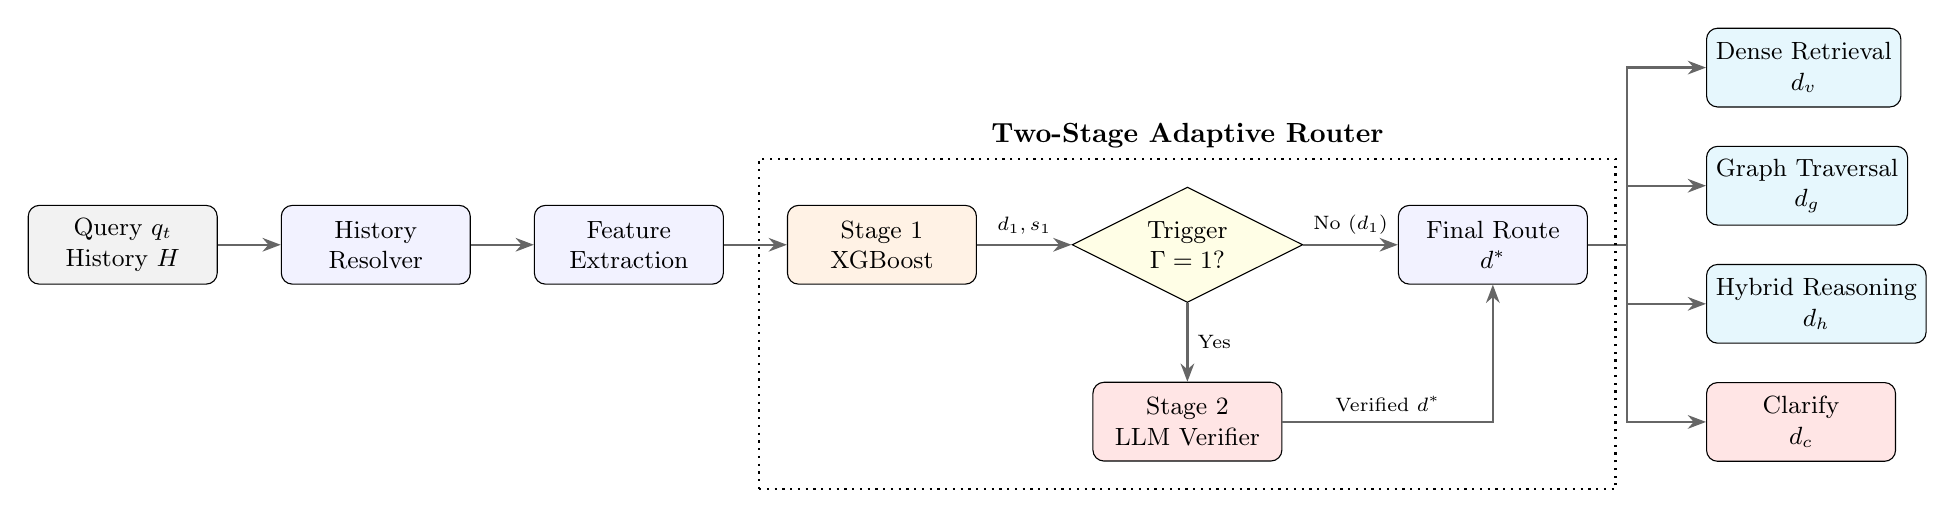
\begin{tikzpicture}[
    node distance=1cm and 1cm,
    box/.style={draw, rectangle, rounded corners, minimum width=2.4cm, minimum height=1cm, align=center, fill=blue!5, font=\small},
    decision/.style={draw, diamond, aspect=2, minimum width=2.5cm, align=center, fill=yellow!10, font=\small},
    arrow/.style={-{Stealth[scale=1]}, thick, draw=gray!80!black},
    label_node/.style={fill=white, inner sep=2pt, font=\scriptsize}
]

    % Input
    \node[box, fill=gray!10] (input) {Query $q_t$ \\ History $H$};
    
    % Features
    \node[box, right=0.8cm of input] (resolver) {History \\ Resolver};
    \node[box, right=0.8cm of resolver] (features) {Feature \\ Extraction};
    
    % Stage 1
    \node[box, fill=orange!10, right=0.8cm of features] (stage1) {Stage 1 \\ XGBoost};
    
    % Trigger
    \node[decision, right=1.2cm of stage1] (trigger) {Trigger \\ $\Gamma=1$?};
    
    % Stage 2
    \node[box, fill=red!10, below=1cm of trigger] (stage2) {Stage 2 \\ LLM Verifier};
    
    % Final Route Decision
    \node[box, right=1.2cm of trigger] (final_route) {Final Route \\ $d^*$};
    
    % Outputs (stacked vertically on the right)
    \node[box, right=1.5cm of final_route, yshift=2.25cm, fill=cyan!10] (dense) {Dense Retrieval \\ $d_v$};
    \node[box, right=1.5cm of final_route, yshift=0.75cm, fill=cyan!10] (graph) {Graph Traversal \\ $d_g$};
    \node[box, right=1.5cm of final_route, yshift=-0.75cm, fill=cyan!10] (hybrid) {Hybrid Reasoning \\ $d_h$};
    \node[box, right=1.5cm of final_route, yshift=-2.25cm, fill=red!10] (clarify) {Clarify \\ $d_c$};

    % Connections
    \draw[arrow] (input) -- (resolver);
    \draw[arrow] (resolver) -- (features);
    \draw[arrow] (features) -- (stage1);
    \draw[arrow] (stage1) -- (trigger) node[midway, above, font=\scriptsize] {$d_1, s_1$};
    
    \draw[arrow] (trigger) -- (final_route) node[midway, above, font=\scriptsize] {No ($d_1$)};
    \draw[arrow] (trigger) -- (stage2) node[midway, right, font=\scriptsize] {Yes};
    \draw[arrow] (stage2.east) -| (final_route.south) node[near start, above, font=\scriptsize] {Verified $d^*$};
    
    \draw[arrow] (final_route.east) -- ++(0.5,0) |- (dense.west);
    \draw[arrow] (final_route.east) -- ++(0.5,0) |- (graph.west);
    \draw[arrow] (final_route.east) -- ++(0.5,0) |- (hybrid.west);
    \draw[arrow] (final_route.east) -- ++(0.5,0) |- (clarify.west);
    
    % Grouping for router
    \node[draw, dotted, thick, inner sep=10pt, fit=(stage1)(trigger)(stage2)(final_route), label={[font=\bfseries]above:Two-Stage Adaptive Router}] (router_box) {};

\end{tikzpicture}
\end{document}
